\NeedsTeXFormat{LaTeX2e}
\documentclass[10pt,a4paper]{scrartcl}

\usepackage{tabularx,graphicx,setspace}

\ifx\pdfoutput\undefined
  % We're not running pdftex
  % european (better) fonts -- does not look good with pdflatex
  \usepackage[T1]{fontenc}
  \newcommand{\href}[2]{#2\\{\hspace*{5mm}\scriptsize <#1>}\\}
\else
  \pdfcompresslevel=9
  \def\pdfBorderAttrs{/Border [0 0 0] } % No border around Links
  \usepackage{hyperref}
\fi

\title{An Analysis of Parallel Rendering Systems}
\author{Stefan Eilemann\thanks{eilemann@gmail.com}\\[\medskipamount]
%  EyeScale Software Sarl
}
\date{}

\newcommand{\tm}{\texttrademark~}
\newcommand{\rc}{\raise 1ex\hbox{{\tiny\textregistered}}~}
% suppress  single floating lines on top (widow) and bottom(club)
%  10000 is infinity
%  tradeoff: maybe underfull vboxes
\clubpenalty=10000
\widowpenalty=10000 

\oddsidemargin .5cm
\evensidemargin .5cm
\topmargin 1cm
\setlength{\textwidth}{15cm}
\setlength{\textheight}{20cm}
\begin{document}

% paragraph spacing -- should be rubber length
%\setlength{\parskip}{\baselineskip}
% paragraph indention for the first line
%\setlength{\parindent}{0em}

\maketitle
\thispagestyle{empty}
% \begin{figure}[ht]
% \centering
% 
\includegraphics[width=5em]{logo.pdf}
% \end{figure}
\vfill
\abstract{
  This White Paper analyzes and classifies the different approaches taken
  to parallel, interactive rendering. The purpose is to clarify common
  misconceptions and false expectations of the capabilities of the
  different classes of parallel rendering software.
  
  We examine the rendering pipeline of the typical visualization
  application and identify the typical bottlenecks found in this
  pipeline. The methods used for parallel rendering are classified in
  three fundamental approaches and then analyzed with respect to their
  influence on this rendering pipeline, which leads to conclusions about
  possible performance gains and the necessary porting effort.
  
  We advocate the need for a generic, open parallel rendering framework to
  build scalable graphics software. The drawbacks of other existing
  solutions are outlined, and a full software stack for graphics clusters
  is proposed. The Equalizer project\footnote{
    \htmladdnormallink{http://www.equalizergraphics.com}
    {http://www.equalizergraphics.com/}} aims to provide such an
  implementation, combining existing software packages with newly
  developed middleware.
}

\vfill
{\center\begin{tabularx}{.88\textwidth}{|l|l|X|}
\hline
\bf Version & \bf Date & \bf Changes \\
\hline
0.6         & January 11, 2007     & Minor rework of the whole paper\\
0.5.2       & September 19, 2006   & Tweaked Figure~\ref{FIG_parallel}\\
0.5.1       & July 5, 2006         & Added link to latest version\\
0.5         & May 19, 2006         & Initial Version\\
\hline
\multicolumn{3}{c}{\footnotesize Latest version at 
  \htmladdnormallink{http://www.equalizergraphics.com/documents/ParallelRenderingSystems.pdf}
  {http://www.equalizergraphics.com/documents/ParallelRenderingSystems.pdf}}\\
\end{tabularx}}
\clearpage
\pagenumbering{arabic}

\section{Introduction}

The purpose of this white paper is to argue for the need for a middleware to
build truely scalable, interactive visualization applications. In
contrast to high-performance computing (HPC), the high-performance
visualization (HPV) community has not generally accepted the need to
parallelize applications for performance. The belief that scalabity can be
achieved transparently by some magic software is still wide-spread, and
contributes to the slow adoption of graphics clusters and virtual reality
installations due to bad application performance and unavailability.

% Definitions

\subsection{Motivation}
% Introduce the topic
Application developers are typically faced with making their applications
aware of multiple graphics cards for two reasons -- either the
application has to run on multipipe display systems, or the rendering has
to be accelerated by using parallel rendering on multiple graphics
cards. The two reasons are not mutually exclusive.

\subsubsection{Multi-View Rendering}
The first motivation is often to run the application on advanced,
multipipe display systems: workstations with multiple monitors, walls
build out of multiple screens or projectors as well as immersive
environments. Such installations need more than one graphics card to
drive all the display systems. Therefore the rendering has to be
distributed across a number of cards, and often across multiple
systems. The outputs of the displays has to be synchronized spatially
and time-wise to provide one coherent image. In immersive environments,
active or passive stereo rendering is a requirement.

\begin{figure}[ht]
\centering
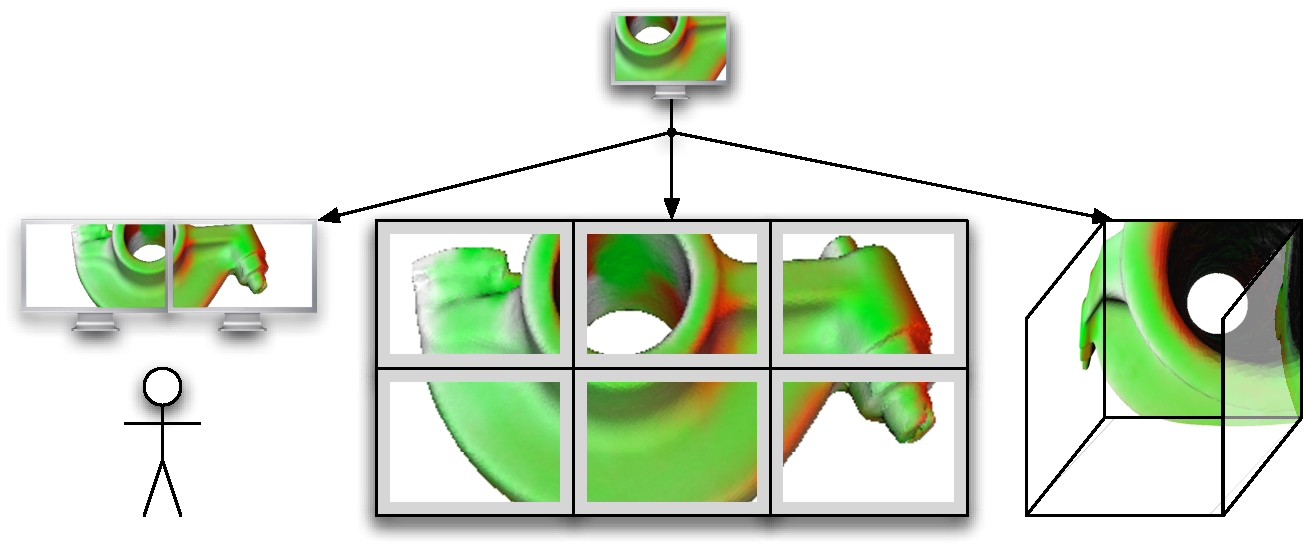
\includegraphics[width=0.9\columnwidth]{images/sp_to_mp.pdf}
\caption{Some advanced display systems}
\label{FIG_multipipe}
\end{figure}

Applications which scale their display size often have to scale
their rendering performance, because the increased display size exposes
previously undiscovered bottlenecks in the rendering pipeline. The higher
display resolution increases the needed pixel fill rate. Due to the increased
image fidelity, data of a higher resolution is used -- which increases
the requirements on the whole rendering pipeline.

\subsubsection{Scalable Rendering}
The second motivation is to accelerate the rendering by aggregating
multiple resources, because the application hits limitations of a single
graphics system. Figure~\ref{FIG_pipeline} shows a simplified rendering
pipeline and the resources used by during rendering. The typical
performance bottlenecks in such a pipeline are:

\begin{figure}[htb]
\centering
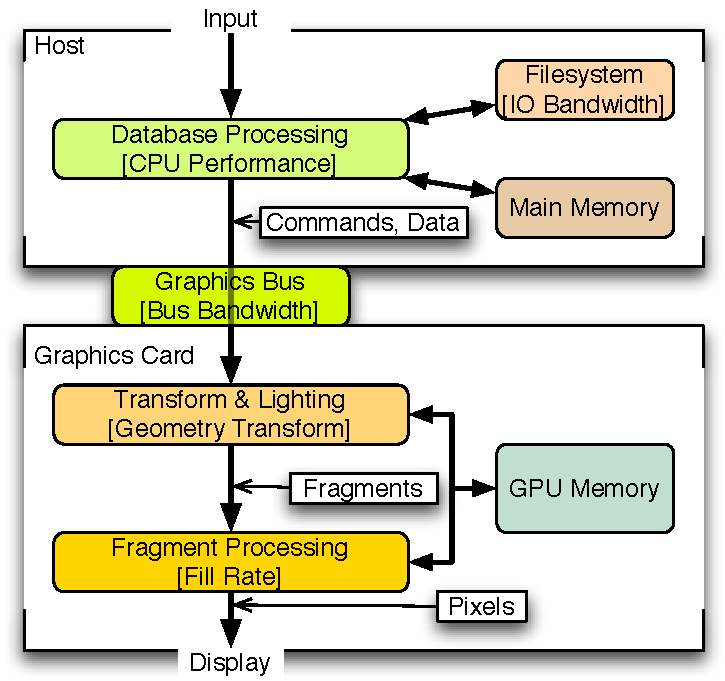
\includegraphics[width=0.45\columnwidth]{images/pipeline.pdf}
\caption{The basic rendering pipeline}
\label{FIG_pipeline}
\end{figure}

\begin{description}
\item[Fill Rate] The amount of rendered pixels can exceed the processing
  capabilities of the graphics card's rasterization pipeline, that
  is, the amount of pixels the card can render in a given time. Volume
  rendering and complex fragment shaders easily limit the application's
  performance due to a fill rate bottleneck.
\item[Geometry Transform] Similar to the fill rate bottleneck, but
  less common, are bottlenecks in the GPU's vertex processing
  capabilities, that is, the amount of triangles a card can
  process. Complex geometry and procedural computations in the vertex
  shader can cause this bottleneck.
\item[GPU Memory] Certain applications, for example volume rendering and
  terrain visualization, easily exceed the amount of memory available on
  the graphics card. For example, a volume of size $1024^3$ has a size
  of 1~GB if it is black and white, and 4~GB if it is colored.
\item[Bus Bandwidth] Dynamic data, such as time-varying data sets and
  interactive modifications of the model, has high requirements on
  the system's IO capabilities. The data can not be cached on the GPU's
  memory but has to be transferred to the card from main memory (or
  disk) during rendering. This is a common bottleneck of interactive
  applications and leads to a rendering performance below the GPU's
  capabilities.
\item[CPU Performance] Similar to the bus bandwidth, the CPU can become
  the bottleneck when traversing the database to generate the rendering
  commands. Tesselation, visibility computations and other
  interpretation of the application data for rendering cause this bottleneck.
\item[Main Memory] The actual model database often holds additional
  application-specific information, which is not used for
  rendering. Additionally, the amount of data displayed is drastically reduced
  during rendering to allow interactive framerates. This leads to
  application scenarios where the required main memory size exceeds the
  capabilities of a single system.
\item[IO Bandwidth] Data sets which exceed the main memory size are
  visualized by roaming through the data, that is, a subset of the whole
  data set is loaded into main memory to be processed and rendered. As
  the user roams through the data, new pieces of it are loaded from
  storage, which can be a bottleneck.
\end{description}


\subsubsection{Parallelism in Graphics Hardware}
Graphics cards address some bottlenecks through hardware
parallelism. GPU's have multiple vertex pipelines (geometry
transform) and multiple fragment pipelines (fill rate) which
accelerate the fill rate and geometry transform rate in hardware,
transparently to the application. Due to physical limitations, the
number of vertex and fragment shading pipelines on a single GPU is limited.

Recent implementations of multi-GPU systems (nVidia SLI, ATI CrossFire)
provide additional parallelism. The individual graphic processors
produce a partial image which is then composited using the hardware
support. The individual GPU's can sit on the same card, or on separate
cards with a special connection between them.

In such a setup, the graphics library dispatches the rendering commands to all
rendering units, a process which is transparent to the application. The overall
pixel fill rate is increased, while other potential bottlenecks are not
addressed, since all commands are sent to all cards and each card needs to
have a copy of all the data (textures, display lists, etc.). A special
case is the alternate frame rendering (AFR) mode,
where each card renders full, alternating frames. This mode also scales
geometry transform and bus bandwidth, while increasing the latency
between input and the rendered output.

Since the application is unmodified, all rendering commands are still
submitted by one thread, which has to be able to saturate the additional
graphics cards to make use of the additional hardware. Distributed scene
graphs and parallel rendering frameworks can in theory parallelize the
rendering for such hardware, once the hardware vendors provide the
necessary API's to program the hardware.

\section{Transparent Multipipe Rendering Software}
% Technical Overview
Transparent rendering software replaces the system's rendering library,
e.g. OpenGL or Direct3D, with a new 'intercept' library. The
application's output is taken at the rendering command level, that is,
the entry points of the rendering library are replaced by new
functions. The new functions package the rendering command stream,
analyze it and send it to a number of rendering processes, potentially
over the network to other systems. This approach is typically used for
the applications which want to use multiple graphics cards to scale the
display size. A limitation of this approach is that unmodified
applications may not be able to run on non-planar display systems,
because important data is not rendered due to the application's view
frustum culling.

% Bottlenecks
Transparent solutions can only increase the rendering performance if the
main bottleneck is on the graphics card (geometry transform or fill rate). The
processing stages to produce the rendering commands are untouched and
remain single-threaded. Potential CPU bottlenecks in the rendering
thread are amplified, since packaging and sending of the rendering
commands to other processes is more time-consuming than writing the
commands directly to a GPU. The bandwidth and latency to the rendering
nodes is worse than the direct local connection to the graphics card. In
reality, this approach often scales the display size at the expense of
performance, since applications are rarely limited by the GPU
processing speed.

% Possible Optimisations
Analyzing the command stream allows some optimizations. The transparent
library can determine the visiblity of rendering commands and textures for each
rendering unit, and only send the data to the appropriate processes.
This can reduce the rendering load of the individual graphics
cards. However, this command stream filtering is only benefitial for the
performance if it can be performed faster than the actual rendering --
which is normally only the case for static chunks of data, such as display
lists and large textures. % mention OpenGL state tracking?

% Parallel Extensions
Some transparent rendering packages support parallelization of the
application, that is, the application is modified and renders using
multiple threads. This support is often rudimentary and does not address other
problems, such as configuration and data distribution. Furthermore, by
working on the low-level graphics command stream, the attainable
performance is limited up-front. From an application developers point of
view, writing a parallel application using a transparent framework is at
least the same effort as using a parallel rendering framework. For the
purpose of this white paper, such an extension to a transparent software
can be considered a parallel rendering framework.

\section{Distributed Scene Graphs}
The distributed scene graph approach requires that the application uses
the given scene graph to describe the model database. The rendering of
that scene graph is parallelized by the scene graph's implementation, to
a great extend transparently to the application. The scene graph is
replicated and kept up-to-date on all rendering nodes. During rendering,
the individual instances are traversed in parallel to generate the
rendering commands, which are directly send to the graphics hardware.

From the applications point of view, this approach is similar to the
transparent solutions, in that the rendering is parallelized by some
'magic' software. The big difference is that a distributed scene graph
approaches the problem at a much higher level, which allows significant
optimizations and leads to better performance. In contrast to
transparent rendering software, the traversal to generate the rendering
commands is parallelized, and the commands are send --in parallel--
directly to the graphics card. The scene graph frees the application
developer of the task to parallelize the rendering.

\section{Parallel Rendering Frameworks}
Parallel rendering frameworks help application developers to parallelize
their application. They do not impose a scene graph or other rendering
libraries on the application. By solving the common problems of
any multiple application, the application developer can focus on
application-specific problems. Parallel rendering frameworks address
synchronization, task decomposition and load-balancing, data transport
as well as the composition of the rendering result. In many ways, they
are  comparable to HPC libraries such as MPI and PVM, while being
focused on interactive applications and parallel rendering.

Parallel rendering frameworks provide an execution environment for any
application, regardless of the used rendering software. Refactoring the
application, other then necessary for multipipe rendering, is not
needed. The application provides entry points for its rendering
functions. Depending on the current configuration, the framework creates
the necessary rendering threads which are initialized with a rendering
context by the application's init functions. When the application
request a new frame of rendering, the framework calls the necessary
rendering callbacks in the correct context and order.

\section{Conclusion}

From a technical point of view, choosing the right approach to
parallel rendering depends on the requirements and bottlenecks of the
application. Figure~\ref{FIG_parallelism} gives an overview how well the
different bottlenecks can be addressed with the various solutions.

\begin{figure}[ht]
\centering
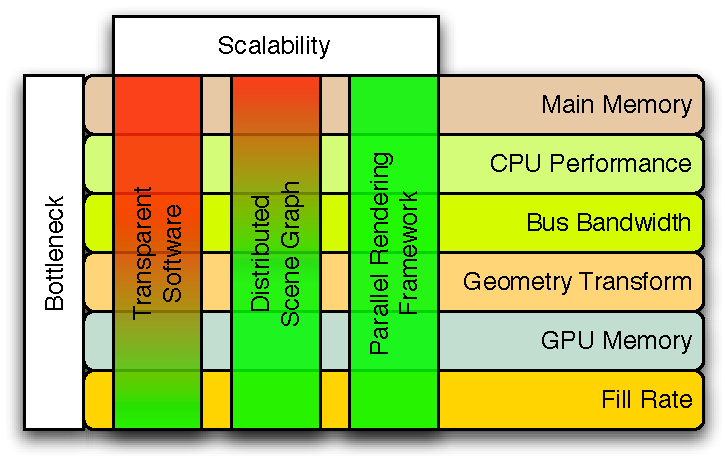
\includegraphics[width=0.45\columnwidth]{images/parallelism.pdf}
\caption{Scalability of the different parallel rendering approaches}
\label{FIG_parallelism}
\end{figure}

% transparent rendering
The least intrusive approach of using a transparent software is often explored
first, which frequently does not meet the expectations and
requirements. Performance gains with transparent solutions are 
possible with benchmarks or well-behaved applications, but
real-world software often does not run faster, slowdowns are commonly
observed. Transparent rendering software often supports only a subset of
the features and extensions of the rendering API, in particular anything
which requires a roundtrip to the graphics card is unsupported or
slow. On the other hand, a transparent solution is a viable way to run a
certain set of applications on graphics clusters. For legacy
applications, which cannot be modified, it is the only possibility to make
them multipipe-ready. The low porting effort is a strong benefit for
transparent rendering software.

% distributed scene graphs
Distributed scene graphs are the ideal and obvious solution if the
application already uses such a scene graph, or is planning on using
one in the near future. The distributed scene graph, especially when
build upon a parallel rendering framework, can deliver optimal
performance while requiring little to no application changes. Porting an
existing application to a distributed scene graph is often impractical
due to the high porting cost.

% parallel rendering frameworks
Parallel rendering frameworks are the common middleware for any
multipipe application. Distributed scene graphs and transparent
rendering software can use it as the base for their
implementation. Applications not suitable for these approaches
can easily implement their parallel rendering on such a framework. The
porting effort is reduced to the unavoidable refactoring needed to
separate the rendering from the core application in order to to make it
distributable. A parallel rendering framework addresses common problems
encountered when doing such a port and follows the natural programming
model for any multipipe application. For high-performance applications,
a parallel rendering framework is the only solution short of a
completely custom implementation.

Parallel rendering frameworks can and should be the foundation of
transparent solutions and distributed scene graphs. These approaches
then become 'applications' of the parallel rendering framework to
address a certain subset of parallel rendering applications - namely
performance-uncritical and legacy applications, as well as applications
already written using a specific scene graph. Figure~\ref{FIG_parallel}
illustrates the proposed software stack.

\begin{figure}[ht]
\centering
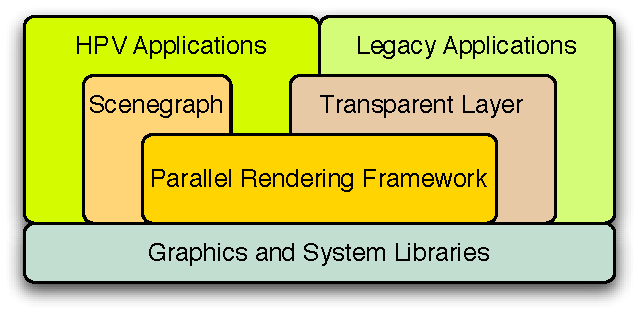
\includegraphics[width=0.45\columnwidth]{images/layers.pdf}
\caption{Proposed software stack for a visualization system}
\label{FIG_parallel}
\end{figure}

% short conclusion.
The three approaches to parallel rendering complement each other and
serve different application needs. Transparent solutions are a quick way
to run interactive applications on graphic clusters, but they do not
provide the necessary performance for many applications. Likewise,
distributed scene graphs are often too invasive since they require the
applications to use a certain format and API --the scene graph-- to
decribe their data. 

\appendix
\section{Current Parallel Rendering Software}
This appendix gives a short and incomplete overview of the existing
software solutions for parallel rendering.

\subsection{Transparent Multipipe Rendering Software}
\subsubsection{Chromium}
Chromium is a Open Source solution originally developed by the
Stanford University. Some graphics cluster vendors, most notably
Tungsten Graphics, support and extend Chromium on their hardware
platforms. Chromium provides functionality for the synchronization
of the rendering commands when using multiple, parallel application
instances.

\subsubsection{VGP Software Solutions}
The Virtual Graphics Platform sold by ModViz, Inc. is a proprietary
software solution similar to Chromium. The VGP Integration API allows to
augment the OpenGL command stream with additional information to improve
the rendering performance.

\subsubsection{OpenGL Multipipe}
OpenGL Multipipe is a transparent software solution delivered with SGI's
multipipe machines. It is not sold separately. For building parallel
applications, SGI offered OpenGL Multipipe SDK.

\subsection{Distributed Scene Graphs}
\subsubsection{TGS Open Inventor Cluster Edition}
The Open Inventor Cluster Edition is an extension to the Open Inventor
scene graph to support parallel, distributed rendering on graphics
clusters. It does support both multi-view and scalable rendering.

\subsubsection{OpenSG}
OpenSG is an open source scenegraph and provides various functionality
for parallel rendering, including network data distribution and scalable
rendering modes.

\subsection{Parallel Rendering Frameworks}
\subsubsection{OpenGL Multipipe SDK}
OpenGL Multipipe SDK from Silicon Graphics, Inc. is a proprietary
framework for the development of scalable graphics applications. It does
not support distributed rendering, and is not actively developed anymore.

\subsubsection{CAVELib}
CAVELib from VRCO Inc. is a proprietary, parallel rendering framework
which supports parallel multi-view rendering.

\subsubsection{Equalizer}
Equalizer is an open source parallel rendering framework under development
by the University of Z\"urich and others. Equalizer supports multi-view
and scalable rendering, and a resource management system and a
transparent rendering layer is planned.

\vfill
\begin{spacing}{.5}{\footnotesize
OpenGL, Open Inventor and OpenGL Multipipe is a trademark of Silicon
Graphics, Inc. SLI is a trademark of nVidia. CrossFire is a trademark of
ATI. Virtual Graphics Platform is a trademark of ModViz, Inc. CAVELib is
a trademark of VRCO Inc. All other products named are trademarks of
their respective owners.
}\end{spacing}
\end{document}
